\chapter{Apron design}

	\section{Introduction}
	The apron is the area of an airport where the aircraft are parked, unloaded or loaded, refuelled and boarded. It also has to cover the taxiways and the trajectories that air planes have to take in order to get to the principal taxiways or the station zones.  
	
	Another function that the apron has to full-fill is the creation of a service way that will allow all the different services needed by the plane to get to it and the creation of some waiting positions for them that will not obstacle the manoeuvres of the plane. Last but not least, the connection between air-side and land-side is under the responsibility of the apron. 
	
	Before moving into a more detailed explanation of each part that makes the apron, a general view is going to be attached in order to obtain a general idea of what is the apron.
	
	\begin{figure}[H]
		\centering
		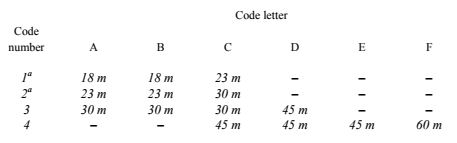
\includegraphics[clip, trim=0cm 0cm 0cm 0cm, width=1\textwidth]{./images/Annex14/RunwayWidth}
		\caption{Runway width according to OACI.} %nom de la figura
		\label{} %per denotar una referencia
	\end{figure}
	
	
	The sections of the apron that will be further explained are the apron taxiways, the aircraft stands, the apron trajectories, service ways and terminal connections. 
	
	\section{Apron taxiways}
	Apron taxiways are designed in order to allow the aircraft to move from the principal taxiway to its specific apron. Due to the fact that our airport has two runways, the number of auxiliary taxiways is higher than a simpler airport. However, ICAO does not have a different criteria for these taxiways. Thus, the parameters and restrictions that apply on the auxiliary taxiways is the same than the principal ones.
	
	Even though the airport is divided in two differenced parts, the domestic flights which have the B737 as most restrictive aircraft and the internationals flights with the B777 as critical air plane, the auxiliary taxiways are designed in order to allow the B777 to operate in the whole airport.
	
	The line that limits the space where aircraft are allowed to taxi is an orange line surrounded by two white lines as it is stated on the ICAO's manual. Since the most restrictive reference letter is E, as it can be seen in the table attached below, the minimum distance between the taxiway's axis is 80m.
	
	\begin{figure}[H]
	\centering
	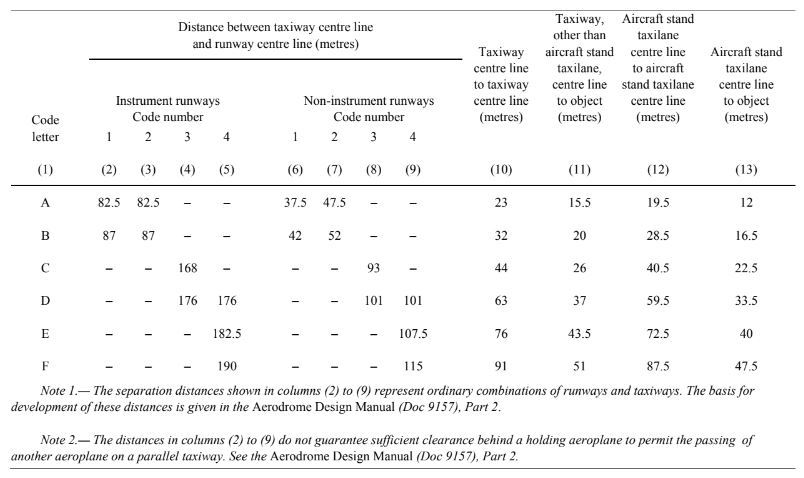
\includegraphics[clip, trim=0cm 0cm 0cm 0cm, width=1\textwidth]{./images/Annex14/minimumdistancetaxiways}
	\caption{Design distances for taxiways according to ICAO.} %nom de la figura
	\label{} %per denotar una referencia
	\end{figure}

	\section{Aircraft stands}
		\subsection{General dimensions of aircraft stands}
		In order to dimension the aircraft stands, the dimensions of the aircraft stated on their ACAP and the ICAO's recommendations have been followed. Starting with the recommendation, the following table shows the distance depending on the reference letter of the air plane. 
		
		\begin{figure}[H]
			\centering
			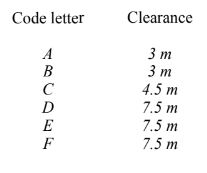
\includegraphics[clip, trim=0cm 0cm 0cm 0cm, width=0.6\textwidth]{./images/Annex14/clearancedistances}
			\caption{Clearance distances depending on the reference letter.} %nom de la figura
			\label{} %per denotar una referencia
		\end{figure}
		
		In order to understand how the aircraft stands are shaped, the following image is attached:
		
		\begin{figure}[H]
			\centering
			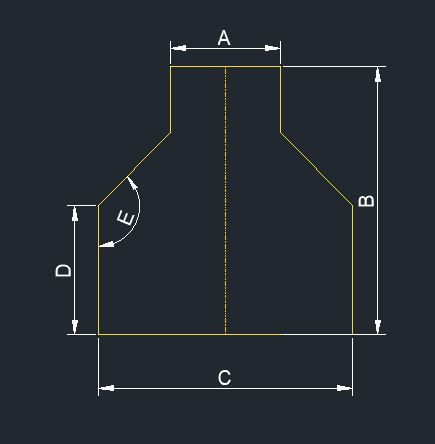
\includegraphics[clip, trim=0cm 0cm 0cm 0cm, width=0.6\textwidth]{./images/Annex14/aircraftstand}
			\caption{Clearance distances depending on the reference letter.} %nom de la figura
			\label{} %per denotar una referencia
		\end{figure}
		
		The next step is to explain how can each distance be obtained:
		
		- A: this distance can be calculated by adding the maximum width of the air plane and the security margin stated on the table attached above.
		
		- B: It can be dimensioned by adding two times the security margin stated by ICAO's recommendation and the aircraft length. The security margin is considered two times since the distance has to be respected in the front part and the rear part of the air plane.
		
		- C: Once more, this distance can be obtained by adding the security margin on each side and the air plane's span. 
		
		- D: This distance can be calculated picking up the distance form C until the last airfoil and adding the contribution of the security margin.
		
		- E: This distance required is geometrically more complex and can be obtained by creating a parallel line distanced the security margin from the line created from the tip of the last airfoil until the edge of the engine.   
		
		\subsection{Dimensions for reference aircraft}
		Before stating all the distances, a reference point must be set. The centre of coordinates is placed in the nose of the plane, the x-axis is considered positive following the aircraft's direction, the y-axis is considered positive in the direction of the left half-wing and the z-axis is oriented to the ground.  
		
		\subsubsection{B777}
		The dimensions of the air plane B777 are the following:
		
		\begin{table}[htb]
			\centering
			\begin{tabular}{ll p{5cm}}
				\midrule[2pt]
				Span & 64,8m\\
				Length & 73,86m\\
				Length last airfoil& 0,6m \\
				Engine position x & 25,76m\\
				Wing tip coordinate & 49,11m\\
				\bottomrule[2pt]
			\end{tabular}
			\caption{Boeing 777 distances and dimensions.}
			\label{Boeingdistances}
		\end{table}
		
		The security margin used on the B777 according to ICAO's table is 7,5m.
		
		\subsubsection{B737}
		Doing the same for the B737, the table obtained is the following:
		
		\begin{table}[htb]
			\centering
			\begin{tabular}{ll p{5cm}}
				\midrule[2pt]
				Span & 35,79m\\
				Length & 39,47m\\
				Length last airfoil& 2,13m \\
				Engine position x & 13,36m\\
				Wing tip coordinate & 23,88m\\
				\bottomrule[2pt]
			\end{tabular}
			\caption{Boeing 737 distances and dimensions.}
			\label{Boeing737distances}
		\end{table}
		
		The security margin used on the B737 according to ICAO's table is 4,5m.
			
	\section{Apron trajectories}
	
	
	\section{Service ways in apron}
	
	
	\section{Terminal connections}
	